\documentclass{beamer}
\usepackage[orientation=landscape, size=a0, scale=1.4]{beamerposter}
\usepackage[absolute,overlay]{textpos}
\usepackage{multicol}
\usepackage{graphics}
\usepackage{url, enumitem}
\usepackage{amsfonts}
\usepackage{listings}
\usepackage{graphicx}
\usepackage{bm}
\usepackage{tikz}
\usetikzlibrary{fit,positioning}
  \usetheme{CambridgeUS}
    \title[Designator]{Designator}
    \addtobeamertemplate{frametitle}{\vskip0.6ex}{}
\newcommand{\N}{\mathcal{N}}	
\begin{document}

%\begin{block}{\centering \Huge {Title Goes Here}}
%\end{block}
\begin{frame}{\centerline{\Huge Gabriel Doesn't Know How to Refactor Code}}
\begin{textblock}{5}(.15,.85)
\begin{block}{Introduction}
Over the past decade, aesthetics have gained a lot of importance in the decisions companies
make in how they design websites, and user experience is at the core of this trend.  In this paper, we develop a way to automate this process by generating color suggestions based on what we call the "Ugly Duckling" problem: essentially recommending what popular similar websites contain that the input website does not yet have. Using Ugly Duckling, we got results that are consistently better than color recommenders based on more classical techniques such as Naive Bayes, SVM, and Random Forest classification.

It is not immediately clear, however, how to find "similar websites." Especially when the website dabatase is large, diffing a screenshot or even the color histogram of a given input website against thousands or millions of other websites can prove to be a daunting task. This paper applies different sorts of unsupervised clustering including KMeans and Affinity Propagation to solve this problem. Once the website database is clustered, the system can place
any input website into a specific cluster. Diffing the input against all websites in a cluster can be
done much faster than within the whole database, and the system will only have to consider
recommendations that are relevant to that specific cluster. 
\end{block}

\begin{block}{Data}
Our data consists of the 5000 most popular websites on the web drawn from the Alexa database, whose screenshots we got using PhantomJS. To keep the data clean, we purged all uninteresting websites that have only 2 or less colors. For feature vectors, we used both ~7000 dimensional RGB arrays and $D=$~17000 dimensional binned histograms. The binned histograms are color histograms where we place color values into bins of size 10, so that we consider the existence of exactly $D$ colors as opposed to the usual 255 * 255 * 255 which is too large.
\end{block}

\begin{block}{Problem and Error Measuring}
Website data is completely unlabeled and it is not immediately clear what a "good" color recommendation would be. To address this issue, we remove a color $c$ from each website in the test set and ask our system to try to recommend it back. In this framework, recommendation becomes a classification problem that tries to infer $c$ out of ~17000 different possible colors, so throughout the paper we consider both the classification accuracy $\tau$ as a percentage (greater is better, doesn't take into account how distant the colors are) and the mean color recommendation error $\delta$ (lower is better, takes into account how distant the colors are).
$$\tau = \frac{\text{Correct}}{\text{Total}} = \frac{\sum_n I[r_n = c_n]}{n}$$
$$\delta_Y = \sum_n |r_n - c_n|$$
\end{block}


\begin{block}{Approach - The Ugly Duckling Problem}
Our recommendation scheme is based on the Ugly Duckling algorithm: given some input website $x$, we take a list of similar websites $Y$ and find the color not present in $x$ that appears most consistently in $Y$.
We implemented a naive recommendation scheme that first clusters all websites, and then
given some incoming website x, first finds the cluster it belongs to and in that cluster finds the
image that is closest to it (which means finding the one with the smallest difference in
histograms). From there, it recommends adding the color that would bring the two images the
closest.
The approach above completely disregards all but the closest sample in the cluster. We wish to
improve it by answering the "ugly duckling" question. Namely if x is our input and Y is a cluster
of websites, what color appears consistently in Y that does not appear in x?
\end{block}

\begin{block}{Graphical Models}
\begin{figure}
\centering
\begin{tikzpicture}
\tikzstyle{main}=[circle, minimum size = 10mm, thick, draw =black!80, node distance = 16mm]
\tikzstyle{connect}=[-latex, thick]
\tikzstyle{box}=[rectangle, draw=black!100]
\node[main, fill = white!100] (Normal) [above] {$\N$ };
\node[main, fill = white!100] (Color) [above=of Normal] {$C$ };
\node[main] (Web) [right=of Color] {$W$};
\node[main,fill={rgb:red,243;green,243;blue,243}] (WebLessColor) [above=of Web, yshift=15mm, xshift=-10mm] {$W_{c}$};
  \path (Normal) edge [connect] (Color)
  	(Web) edge [connect] (Color)
  	(Color) edge [connect] (WebLessColor)
  	(Web) edge [connect] (WebLessColor);
\end{tikzpicture}
\end{figure}
\end{block}


\end{textblock}

\begin{textblock}{5}(5.5, .85)

\begin{block}{K-Means using Images}
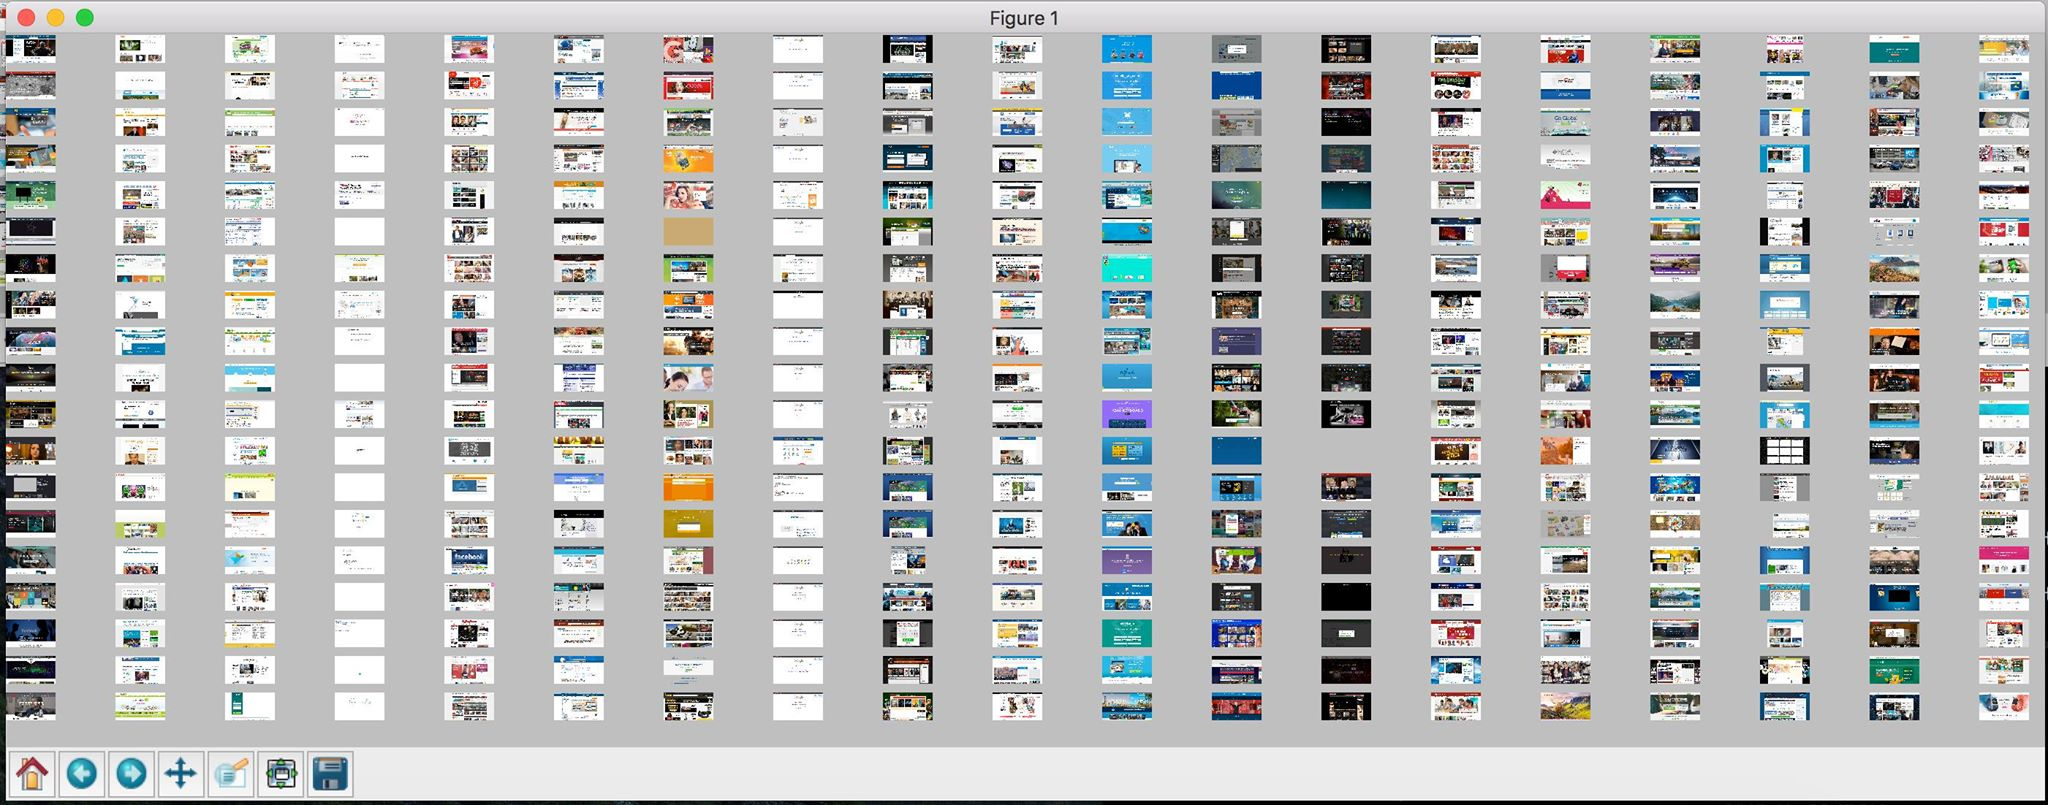
\includegraphics[scale=.5]{imgkmeans.png}
\end{block}
\begin{block}{ K-Means using Binned Histograms}
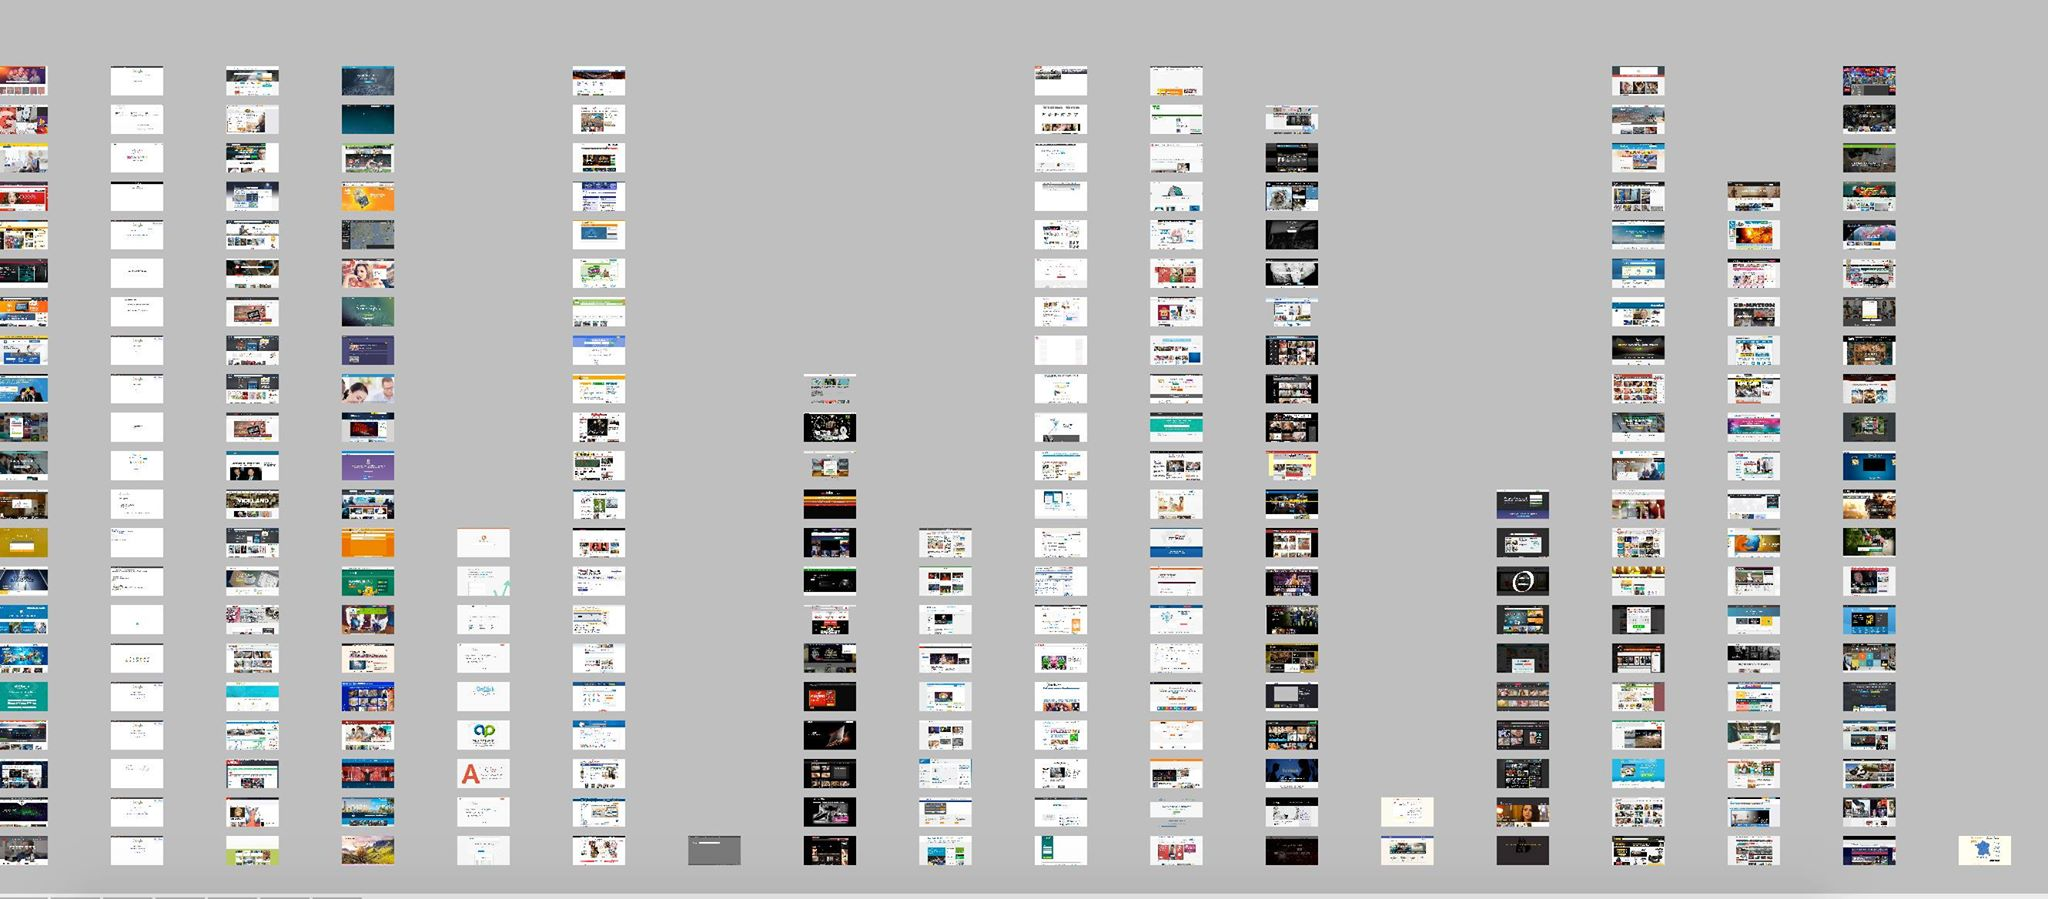
\includegraphics[scale=.5]{binKmeans.jpg}
\end{block}
\begin{block}{Affinity Propogation using Image}
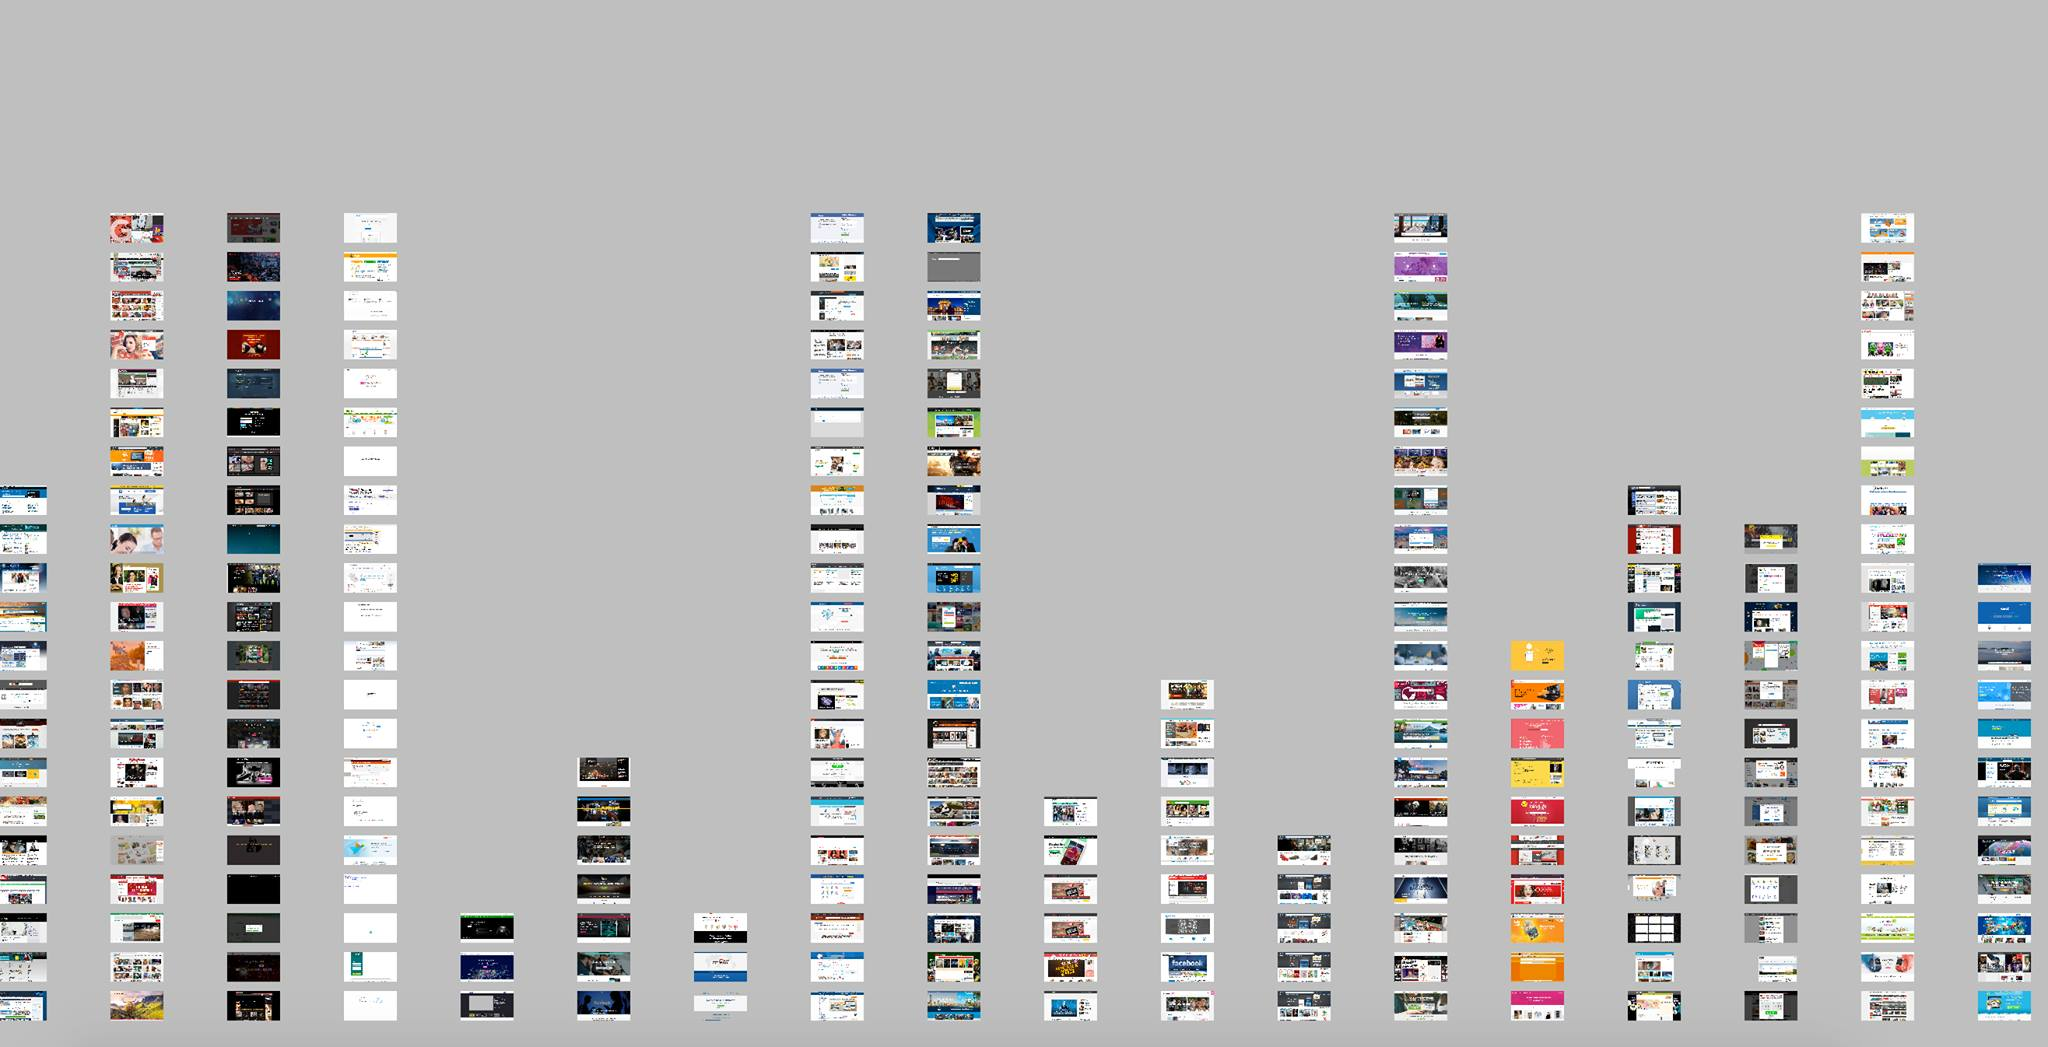
\includegraphics[scale=.5]{affPropImg.jpg}
\end{block}
\begin{block}{Affinity Propogation using Binned Histograms}
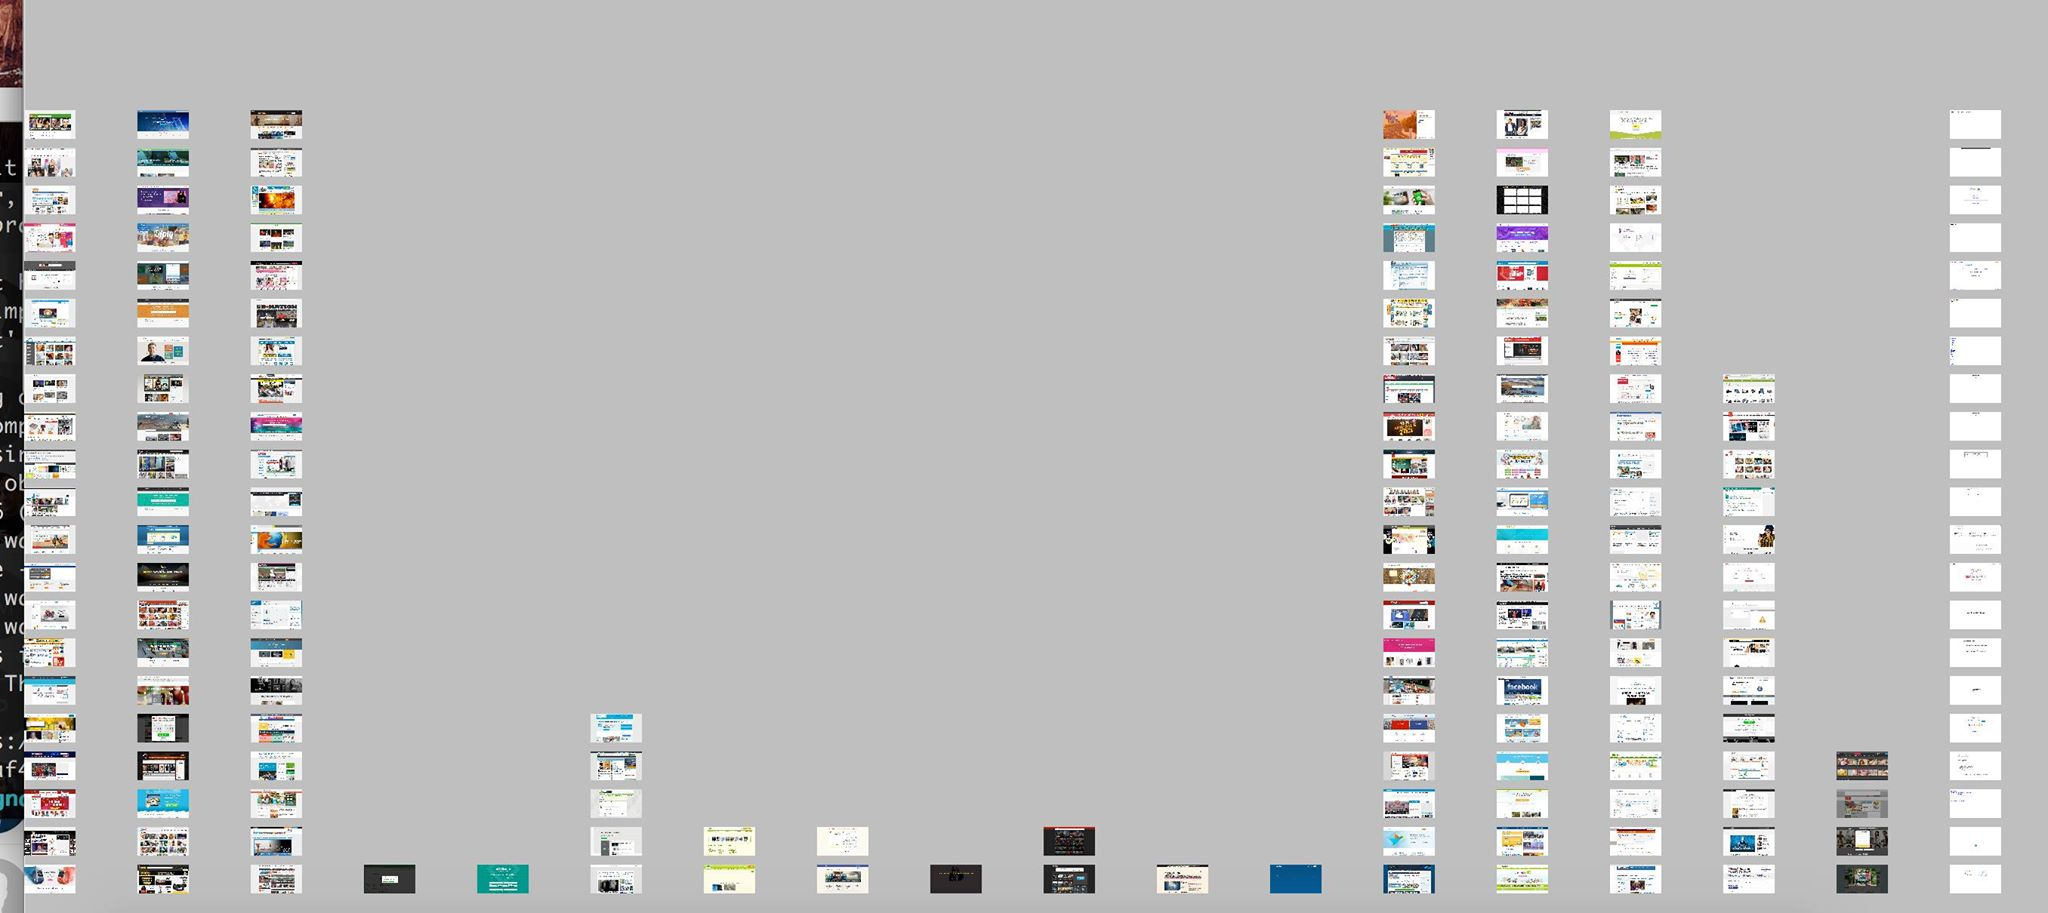
\includegraphics[scale=.5]{binAffProp.jpg}
\end{block}
\end{textblock}

\begin{textblock}{5}(10.75, .85)
\begin{block}{Life Cycle of a Duck}
We initially started recommendations by using K-means (and then Affinity Propogation) clustering to first group our training websites, predicting which cluster our test website belongs to and then running Duckling within that chosen cluster. However, we tried to do something different the next time around: we instead generated clusters for each website on the fly. To do this, we would used the following ratio to calculate similarities between two websites via the following ratio: $\frac{|A \cap B|}{|A \cup B|}$. This ratio is known as the Jaccard index. The higher the ratio, the more similar two sets are. In this case, we chose the websites that had the highest ratios, called that a cluster, and then ran our Duckling recommender on the set for the website.
\end{block}
\end{textblock}
\end{frame}
\end{document}